\newpage

\section{Тестирование системы}

% Тестирование веб-приложений – это комплекс услуг,
% который может включать в себя различные виды тестирования ПО.

% Основная цель любого тестирования,
% в том числе и тестирования веб-приложений, - обнаружить все ошибки в программном обеспечении
% и разработать рекомендации по их предотвращению в будущем.

% \subsection{Тестирование верстки}
% \subsection{Функциональное тестирование}
% \subsection{Usability тестирование (User Experience)}
% \subsection{Тестирование совместимости (конфигурационное тестирование)}
% \subsection{Тестирование производительности}
% \subsection{Тестирование безопасности}
% \subsection{Регрессионное тестирование}

\subsection{Описание входных и выходных данных}

В базе данных MySQL храняться следующие таблицы

\begin{itemize}
    \item \textbf{admins} - таблица для хранения логинов администратора и их захэшированные пароли.
    Скриншот на \textbf{рис.~\ref{fig:gpi_pz_mysql_admins} (стр.~\pageref{fig:gpi_pz_mysql_admins})}.
    \item \textbf{products} - таблица для зранения данных о продукте.
    Скриншот на \textbf{рис.~\ref{fig:gpi_pz_mysql_products} (стр.~\pageref{fig:gpi_pz_mysql_products})}.
\end{itemize}

\begin{figure}[!h]
    \centering
    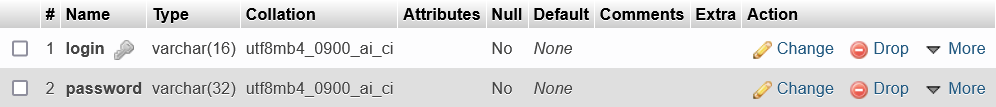
\includegraphics[width=16cm]
        {_assets/gpi_pz_mysql_admins.png}
    \caption{MySQL таблица admins}
    \label{fig:gpi_pz_mysql_admins}
\end{figure}

\begin{figure}[!h]
    \centering
    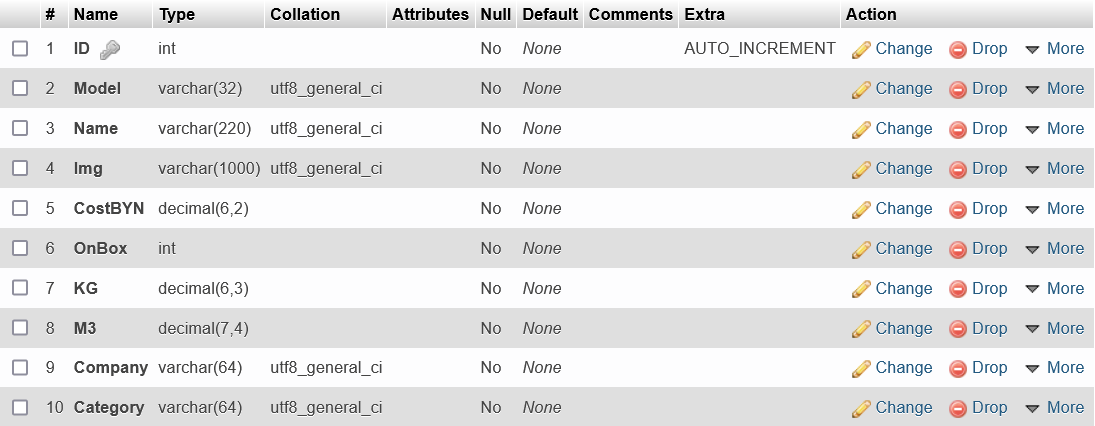
\includegraphics[width=16cm]
        {_assets/gpi_pz_mysql_products.png}
    \caption{MySQL таблица products}
    \label{fig:gpi_pz_mysql_products}
\end{figure}

\newpage

\subsection{Тестирование приложения}

Среда тестирования: 

\begin{itemize}
    \item \textbf{ПК} Acer Aspire 3:
    \begin{itemize}
    \item processor - AMD Ryzen 3 3250U with  Radeon Graphics 2.60 GHz;
    \item installed memory (RAM) - 4.00 (3.44 GB usable);
    \item system type - 64-bit Operating System, x64-based processor.
    \end{itemize}
    \item \textbf{Браузер} Mozilla Firefox 91.4.0esr (64-bit).
    \item \textbf{БД} - MySQL 8.0.27.
    \item \textbf{Виртуальная машина} - Docker 20.10.11, docker-compose 2.2.1.
    \item \textbf{Сборщик проекта} - Make 4.3.
    \item \textbf{Сервер} - Express 4.17.1.
\end{itemize}

% = = = = = = = = = = = = = = = = = = = = = = = = = = = = = = = =

\subparagraph{Тестируемая задача:} <<Авторизация в панели администратора с неверным вводом данных: логина или пароля>>

\textit{Ожидаемый результат}: администратор не авторизуется - сервер отправит результат о не подходящем логине или пароле,
браузер сообщит об ошибке.

\textit{Полученный результат}: администратор не аторизовался, браузер сообщил об ошибке.

\textit{Выводы по тесту}: \\
Скриншот сообщения о несуществовании логина на
\textbf{рис.~\ref{fig:gpi_pz_auth_error_login} (стр.~\pageref{fig:gpi_pz_auth_error_login})}.\\
Скриншот сообщения о неправильном пароле на
\textbf{рис.~\ref{fig:gpi_pz_auth_error_password} (стр.~\pageref{fig:gpi_pz_auth_error_password})}.

\begin{figure}[!h]
    \centering
    \begin{minipage}{0.47\textwidth}
        \centering
        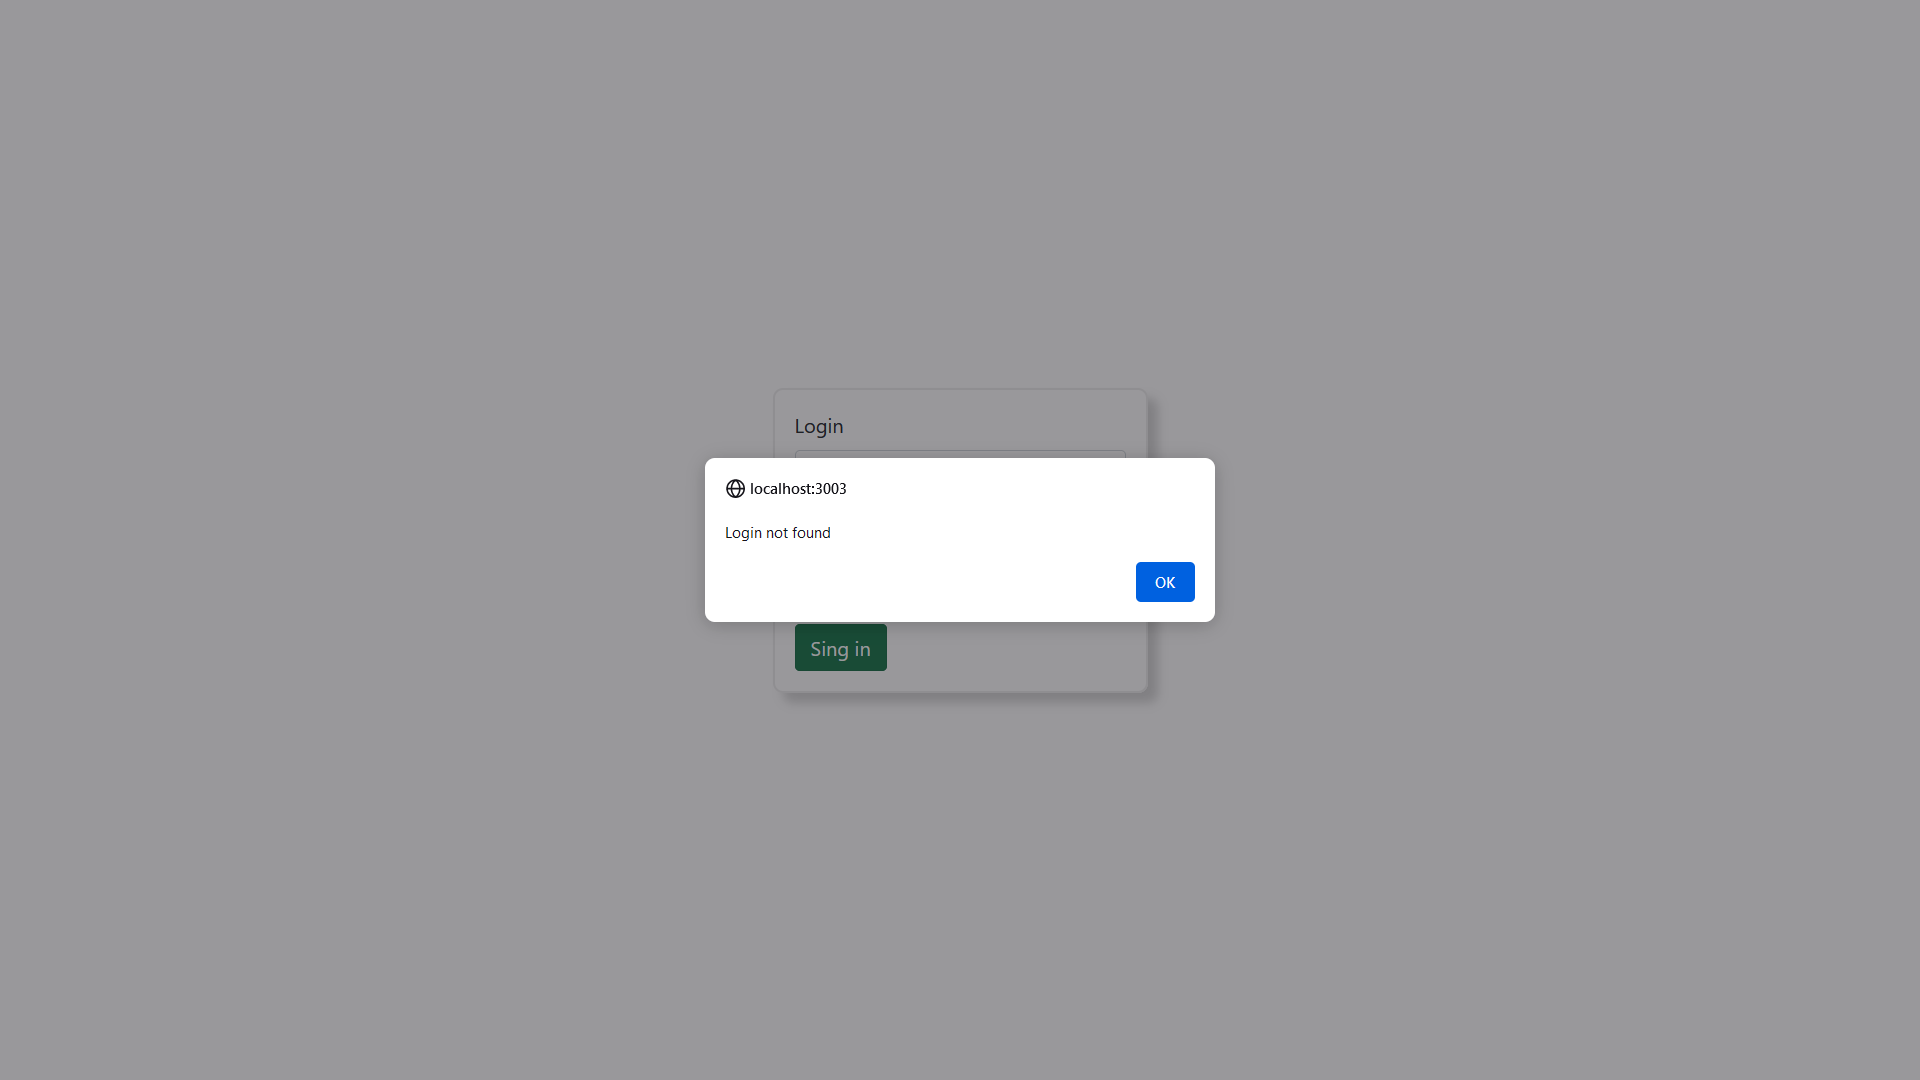
\includegraphics[width=\linewidth]
            {_assets/gpi_pz_auth_error_login.png}
        \caption{Сообщение об несуществовании логина}
        \label{fig:gpi_pz_auth_error_login}
    \end{minipage}
    \begin{minipage}{0.47\textwidth}
        \centering
        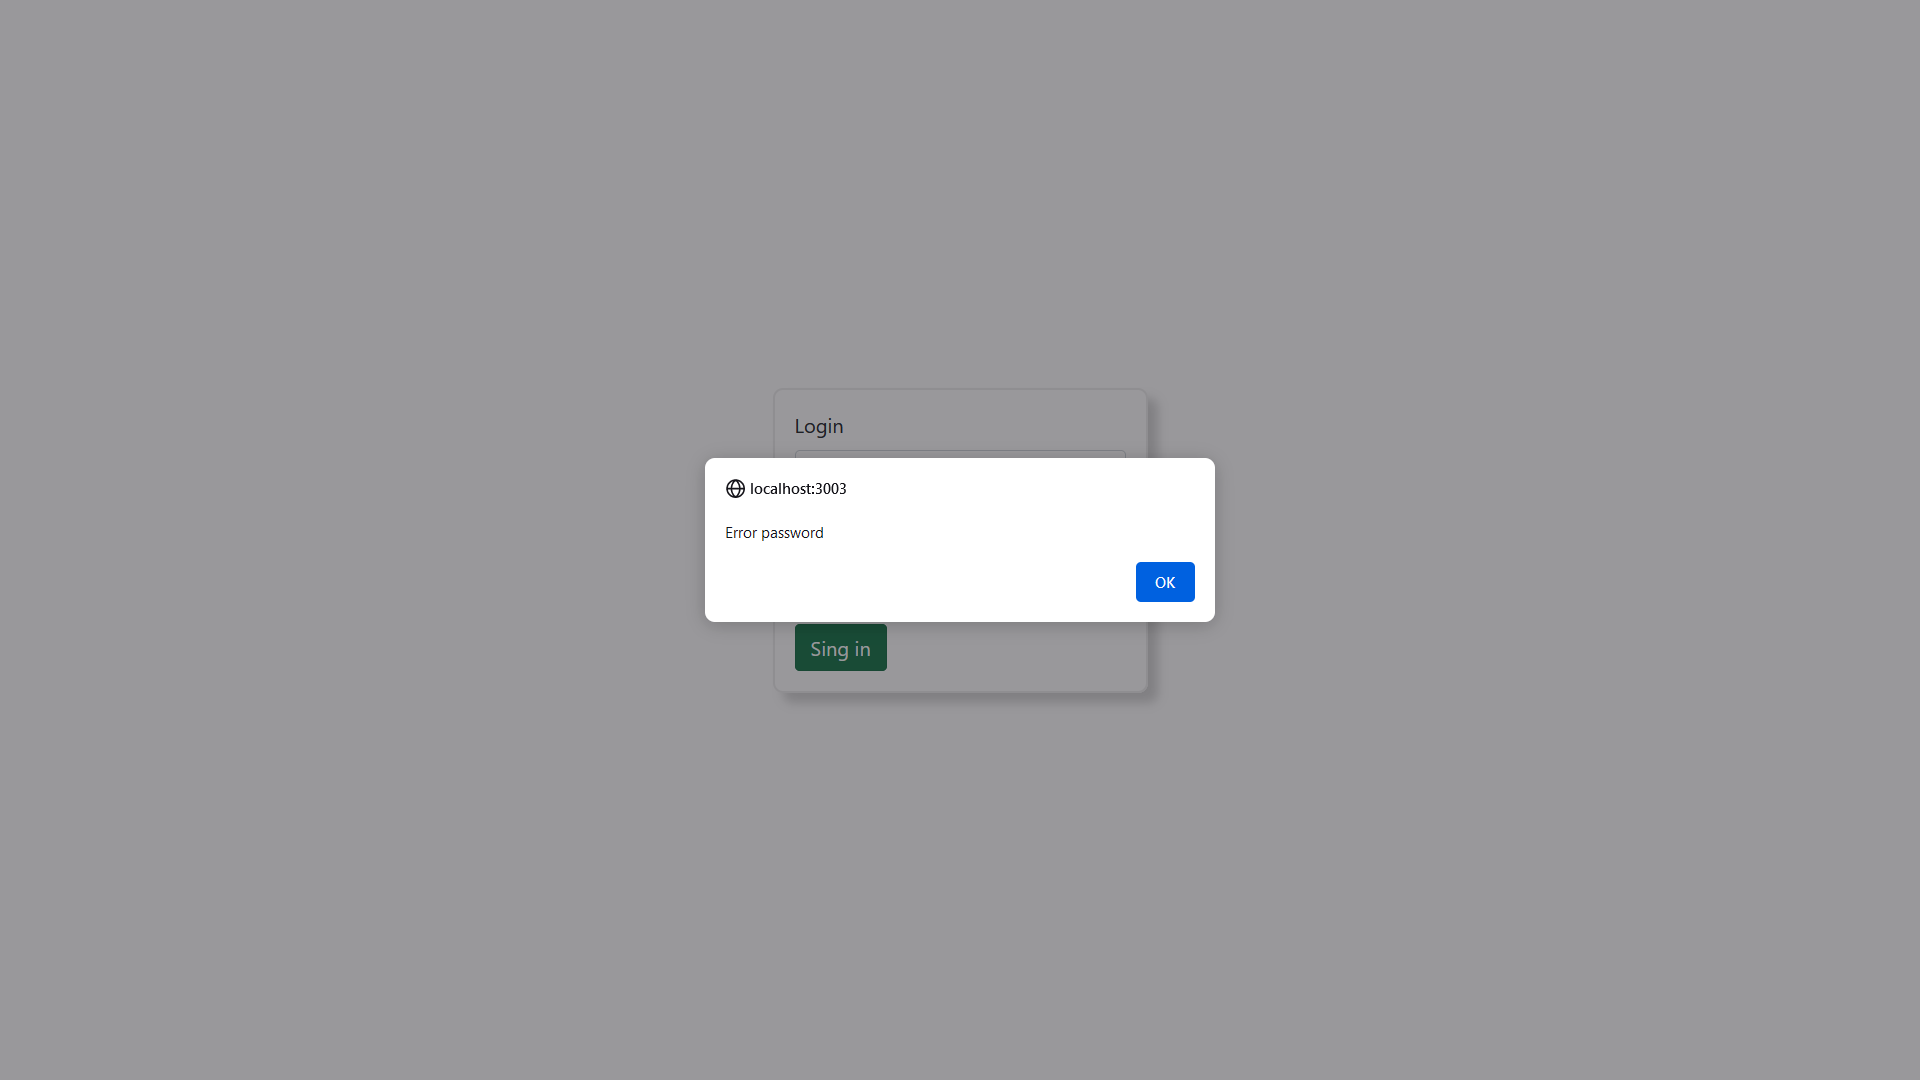
\includegraphics[width=\linewidth]
            {_assets/gpi_pz_auth_error_password.png}
        \caption{Сообщение об неверном пароле}
        \label{fig:gpi_pz_auth_error_password}
    \end{minipage}
\end{figure}

% = = = = = = = = = = = = = = = = = = = = = = = = = = = = = = = =

\subparagraph{Тестируемая задача:} <<Авторизация в панели администратора с верным вводом данных: логин существет и хэш пароля подходит>>

\textit{Ожидаемый результат}: администратор авторизуется - сервер отправит результат об успехе,
браузер перенаправится в админ панель.

\textit{Полученный результат}: администратор авторизовался, браузер перенаправил в админ панель.

\textit{Выводы по тесту}:
Скриншот страницы, на которую перенаправился администратор после успешной авторизации, на
\textbf{рис.~\ref{fig:gpi_pz_adminpanel} (стр.~\pageref{fig:gpi_pz_adminpanel})}.

\begin{figure}[!htb]
    \centering
    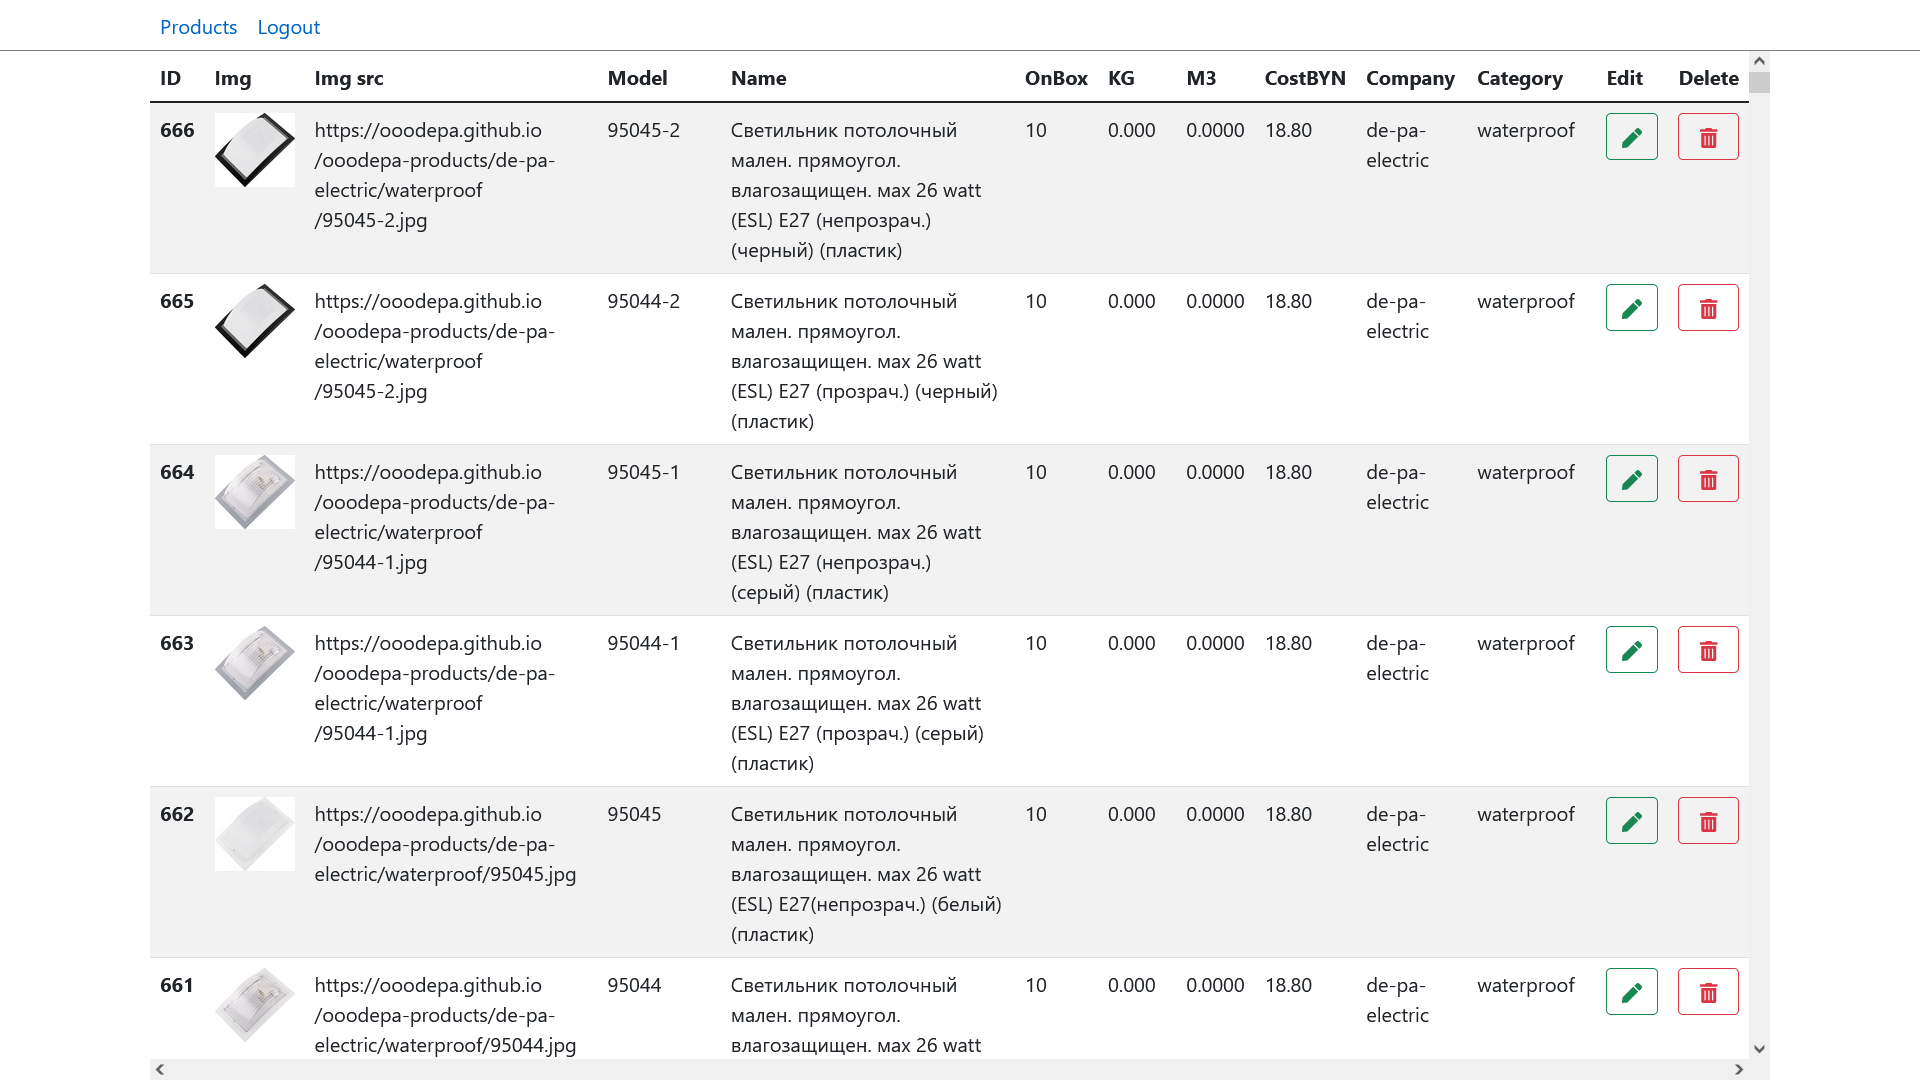
\includegraphics[width=12cm]
        {_assets/gpi_pz_not_empty_table.png}
    \caption{Таблица продуктов после открытия файла}
    \label{fig:gpi_pz_adminpanel}
\end{figure}

% = = = = = = = = = = = = = = = = = = = = = = = = = = = = = = = =

\subparagraph{Тестируемая задача:} <<Открытие текстового файла не JSON формата>>

\textit{Ожидаемый результат}: файл загрузится в браузер, браузер сообщит об ошибке формата файла.

\textit{Полученный результат}: файл загрузился в браузер, браузер сообщил об ошибке формата файла.

\textit{Выводы по тесту}:
Скриншот таблицы после открытия файла на
\textbf{рис.~\ref{fig:gpi_pz_error_open_file} (стр.~\pageref{fig:gpi_pz_error_open_file})}.

\begin{figure}[!htb]
    \centering
    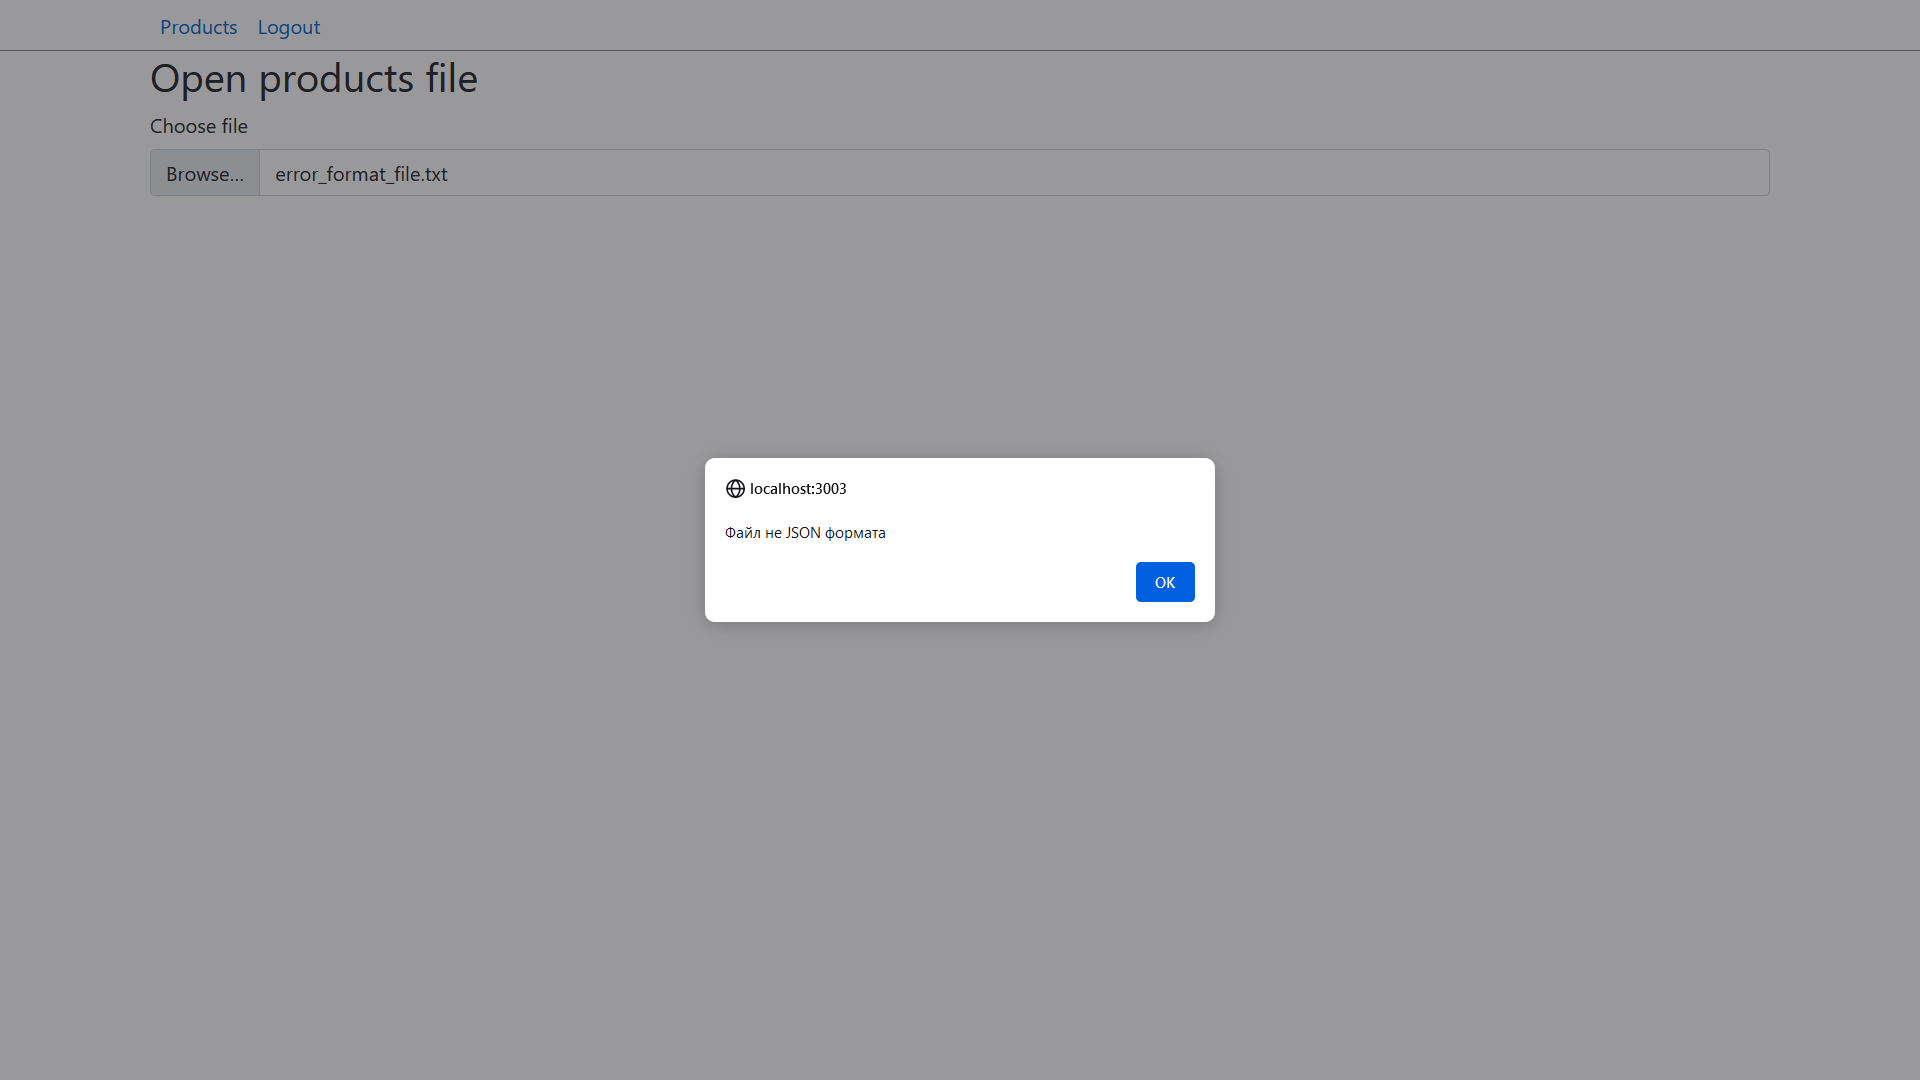
\includegraphics[width=10cm]
        {_assets/gpi_pz_error_open_file.png}
    \caption{Сообщение об не верном текстовом файле (не JSON)}
    \label{fig:gpi_pz_error_open_file}
\end{figure}

% = = = = = = = = = = = = = = = = = = = = = = = = = = = = = = = =

\newpage

\subparagraph{Тестируемая задача:} <<Открытие текстового файла в виде массива структур (JSON)>>

\textit{Ожидаемый результат}: файл загрузится в браузер, браузер перенаправит файл на сервер,
сервер добавит данные в таблицу MySQL и данные можно увидеть в таблице.

\textit{Полученный результат}: файл загрузился в браузер, браузер сообщил об добавленных данных.
На странице таблицы можно увидеть добавленные данные.

\textit{Выводы по тесту}:\\
Скриншот таблицы продуктов до открытия файла на
\textbf{рис.~\ref{fig:gpi_pz_empty_table} (стр.~\pageref{fig:gpi_pz_empty_table})}.\\
Скриншот сообщения о добавлении продуктовиз тектового файла на
\textbf{рис.~\ref{fig:gpi_pz_open_products_json} (стр.~\pageref{fig:gpi_pz_open_products_json})}.\\
Скриншот таблицы продуктов после открытия файла на
\textbf{рис.~\ref{fig:gpi_pz_not_empty_table} (стр.~\pageref{fig:gpi_pz_not_empty_table})}.

\begin{figure}[!h]
    \centering
    \begin{minipage}{0.47\textwidth}
        \centering
        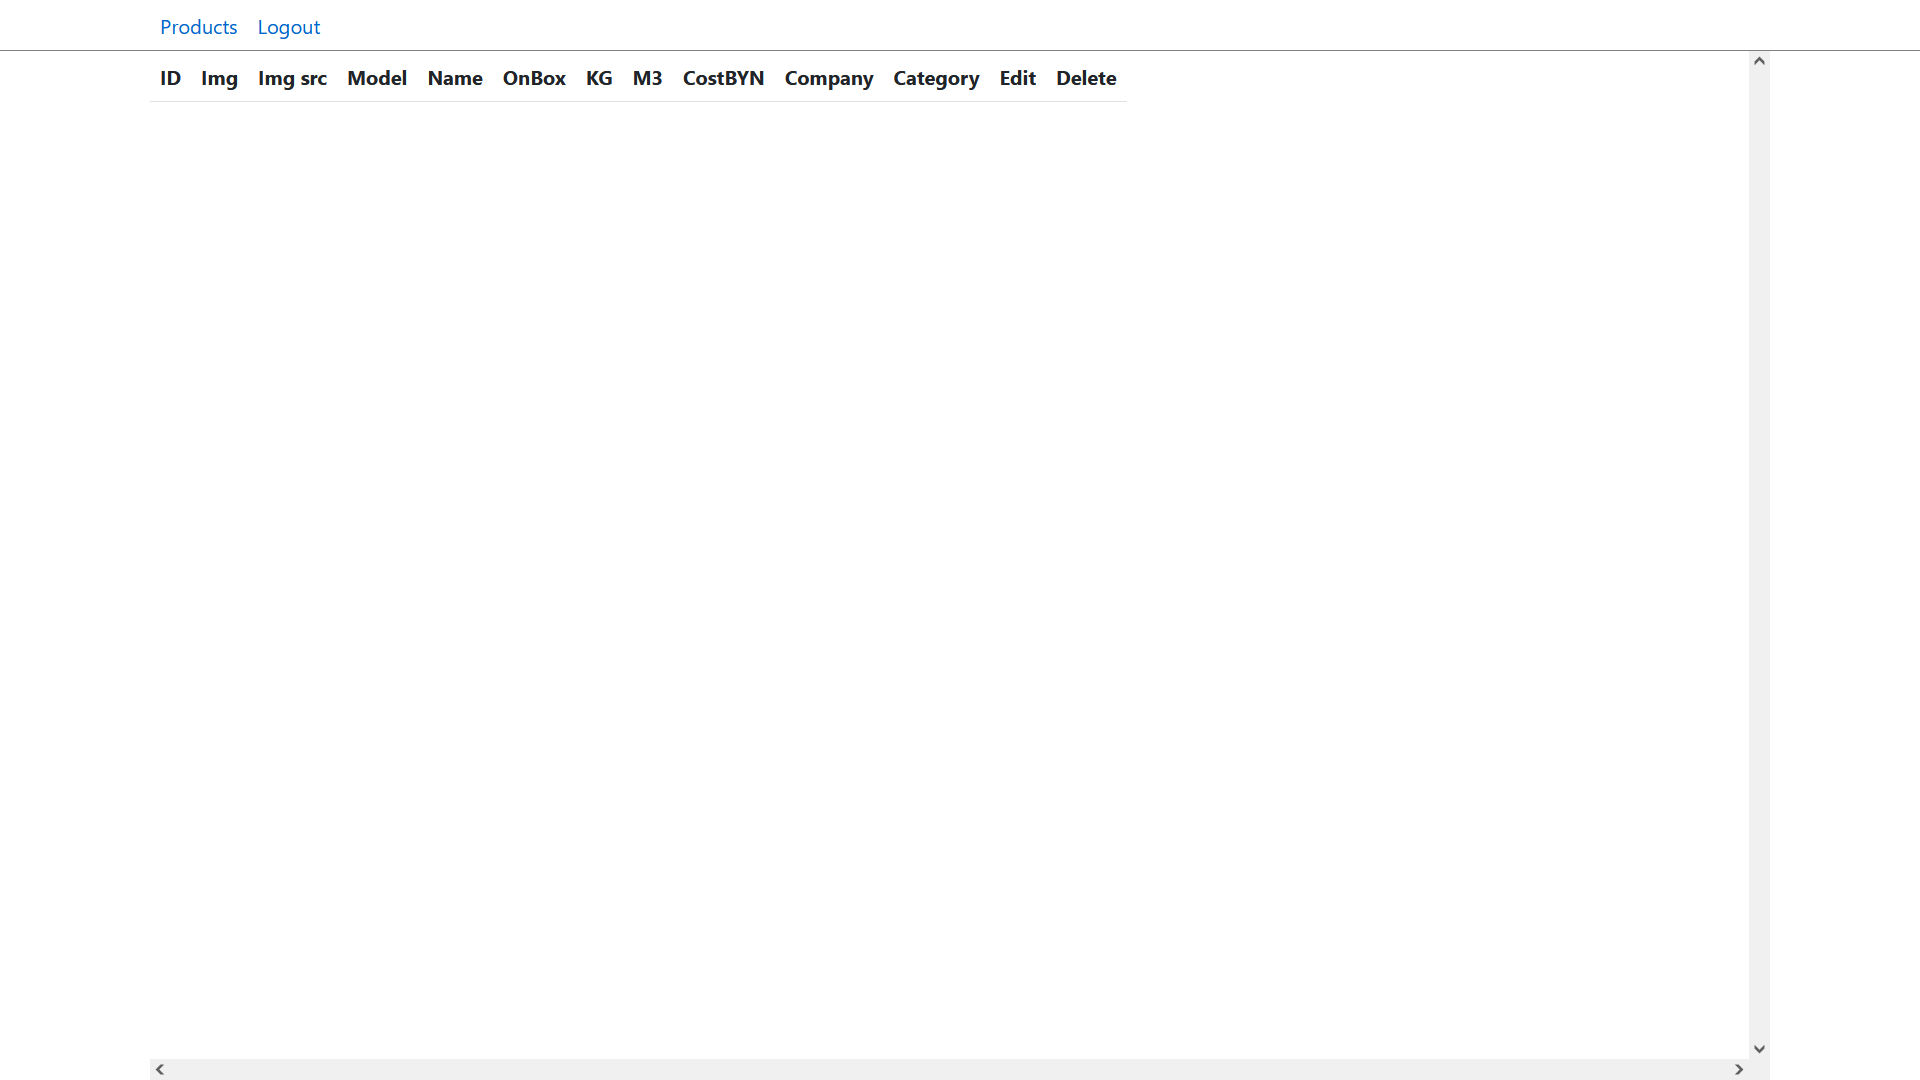
\includegraphics[width=\linewidth]
            {_assets/gpi_pz_empty_table.png}
        \caption{Таблица товаров до открытия файла}
        \label{fig:gpi_pz_empty_table}
    \end{minipage}
    \begin{minipage}{0.47\textwidth}
        \centering
        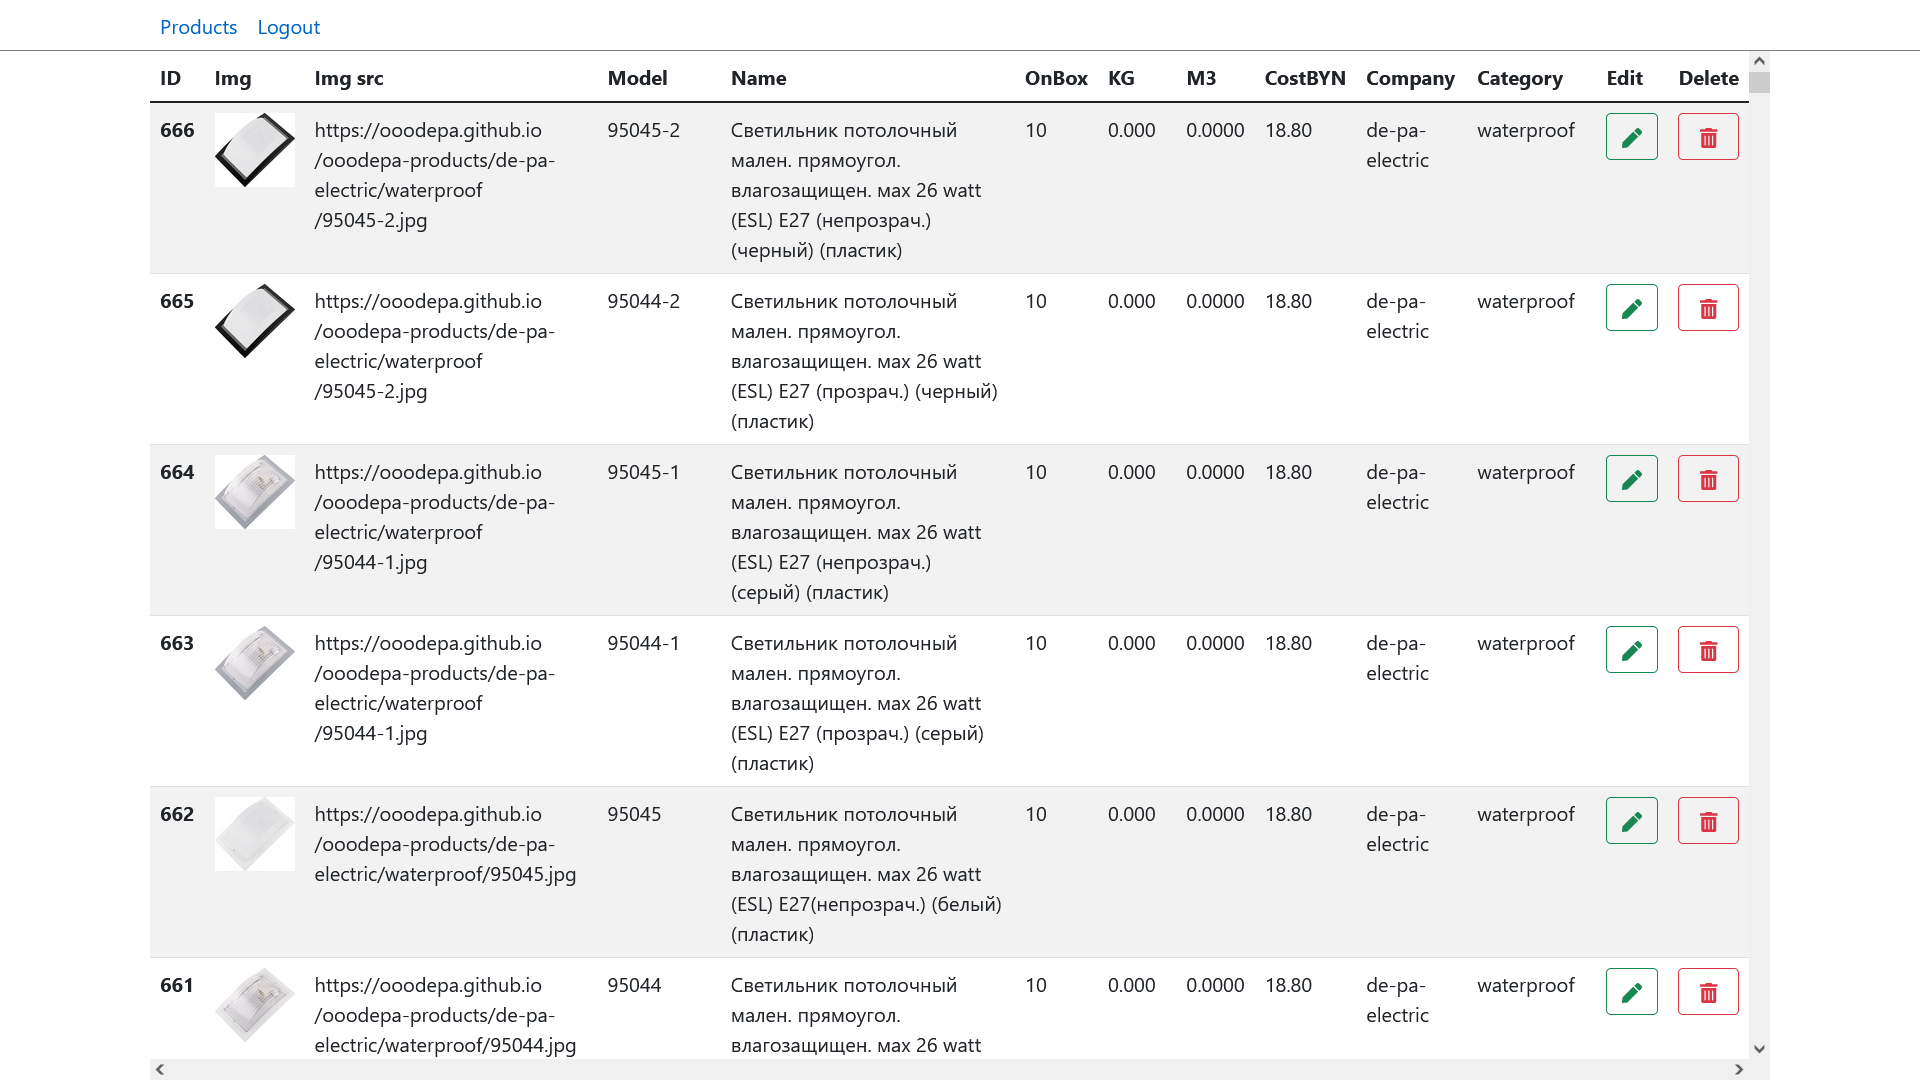
\includegraphics[width=\linewidth]
            {_assets/gpi_pz_not_empty_table.png}
        \caption{Таблица продуктов после открытия файла}
        \label{fig:gpi_pz_not_empty_table}
    \end{minipage}
\end{figure}

\begin{figure}[!htbp]
    \centering
    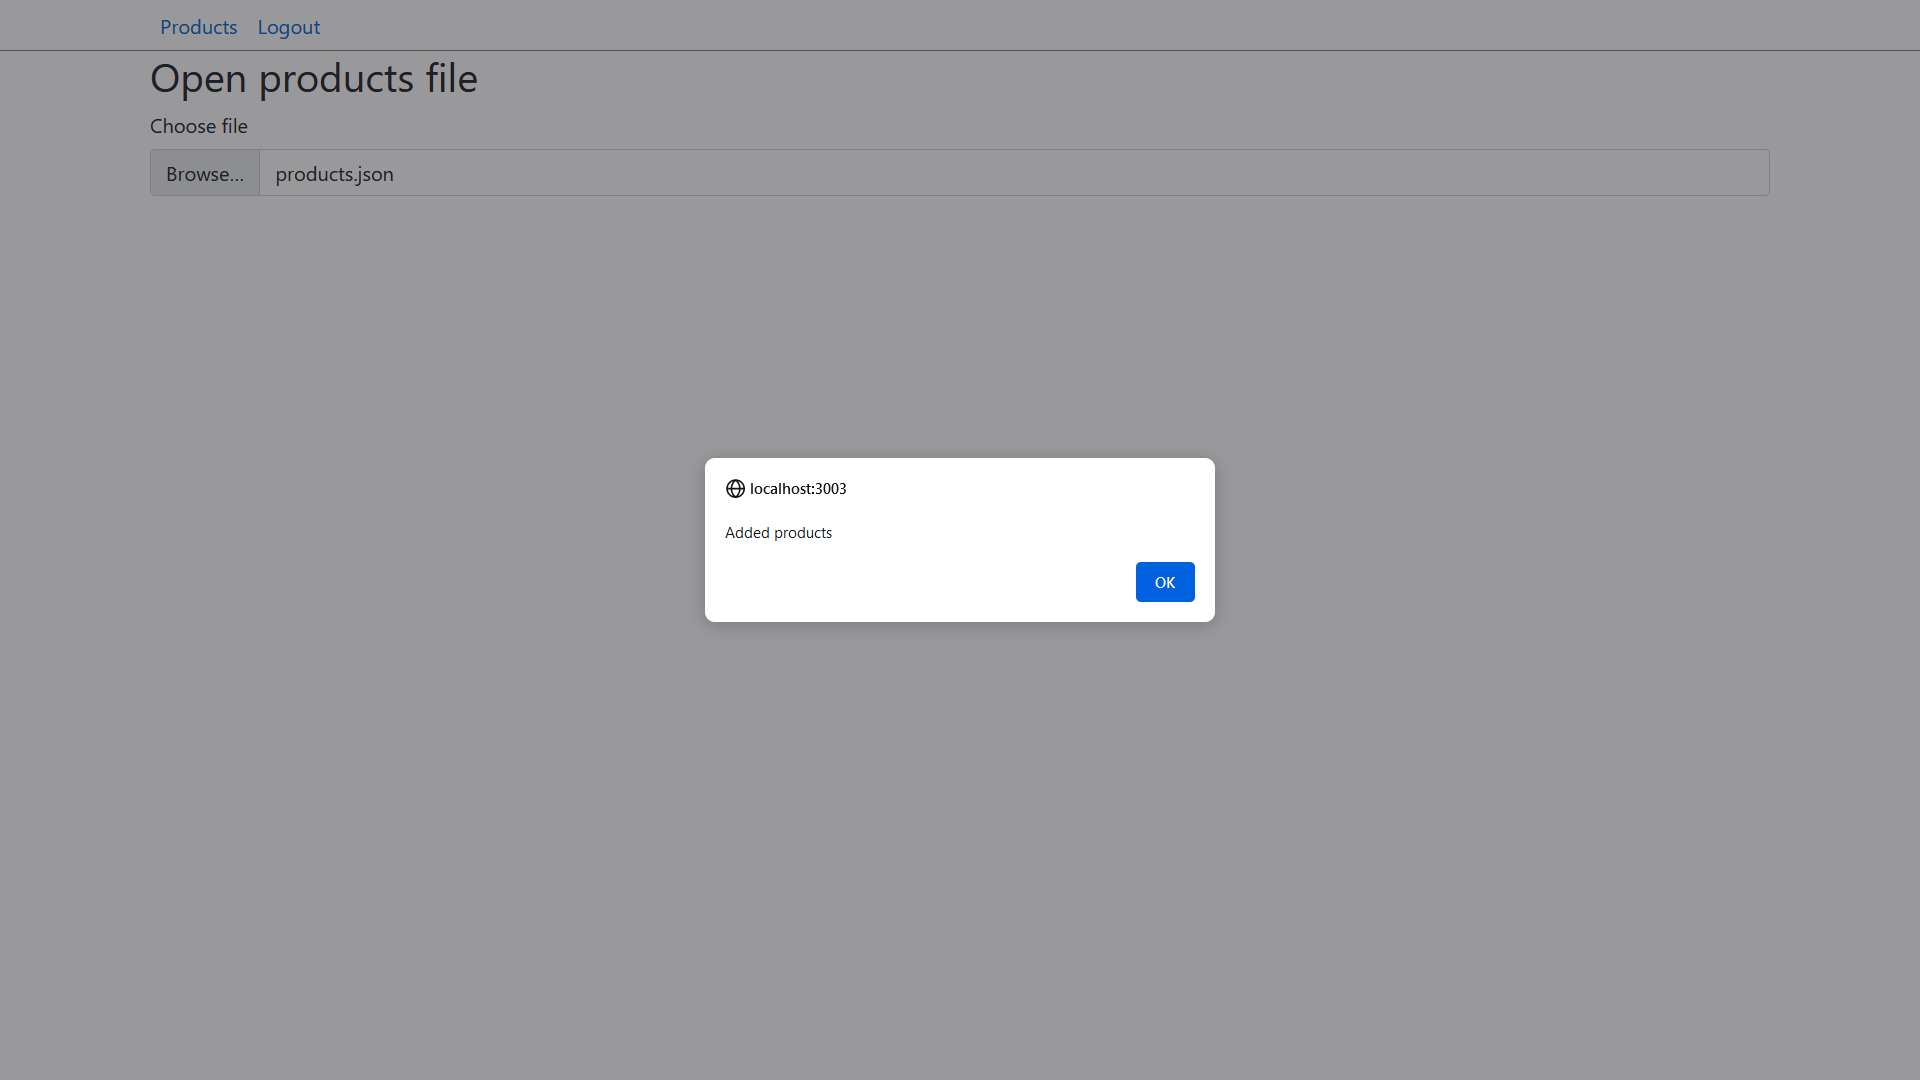
\includegraphics[width=12cm]
        {_assets/gpi_pz_open_products_json.png}
    \caption{Сообщение об добавлении продуктов из текстового файла (JSON)}
    \label{fig:gpi_pz_open_products_json}
\end{figure}

% = = = = = = = = = = = = = = = = = = = = = = = = = = = = = = = =

\newpage

\subparagraph{Тестируемая задача:} <<Просмотр таблицы продуктов>>

\textit{Ожидаемый результат}: выведится таблица продуктов.

\textit{Полученный результат}: вывелась таблица продуктов.

\textit{Выводы по тесту}:
Скриншот таблицы продуктов на
\textbf{рис.~\ref{fig:gpi_pz_products_table} (стр.~\pageref{fig:gpi_pz_products_table})}.

\begin{figure}[!htbp]
    \centering
    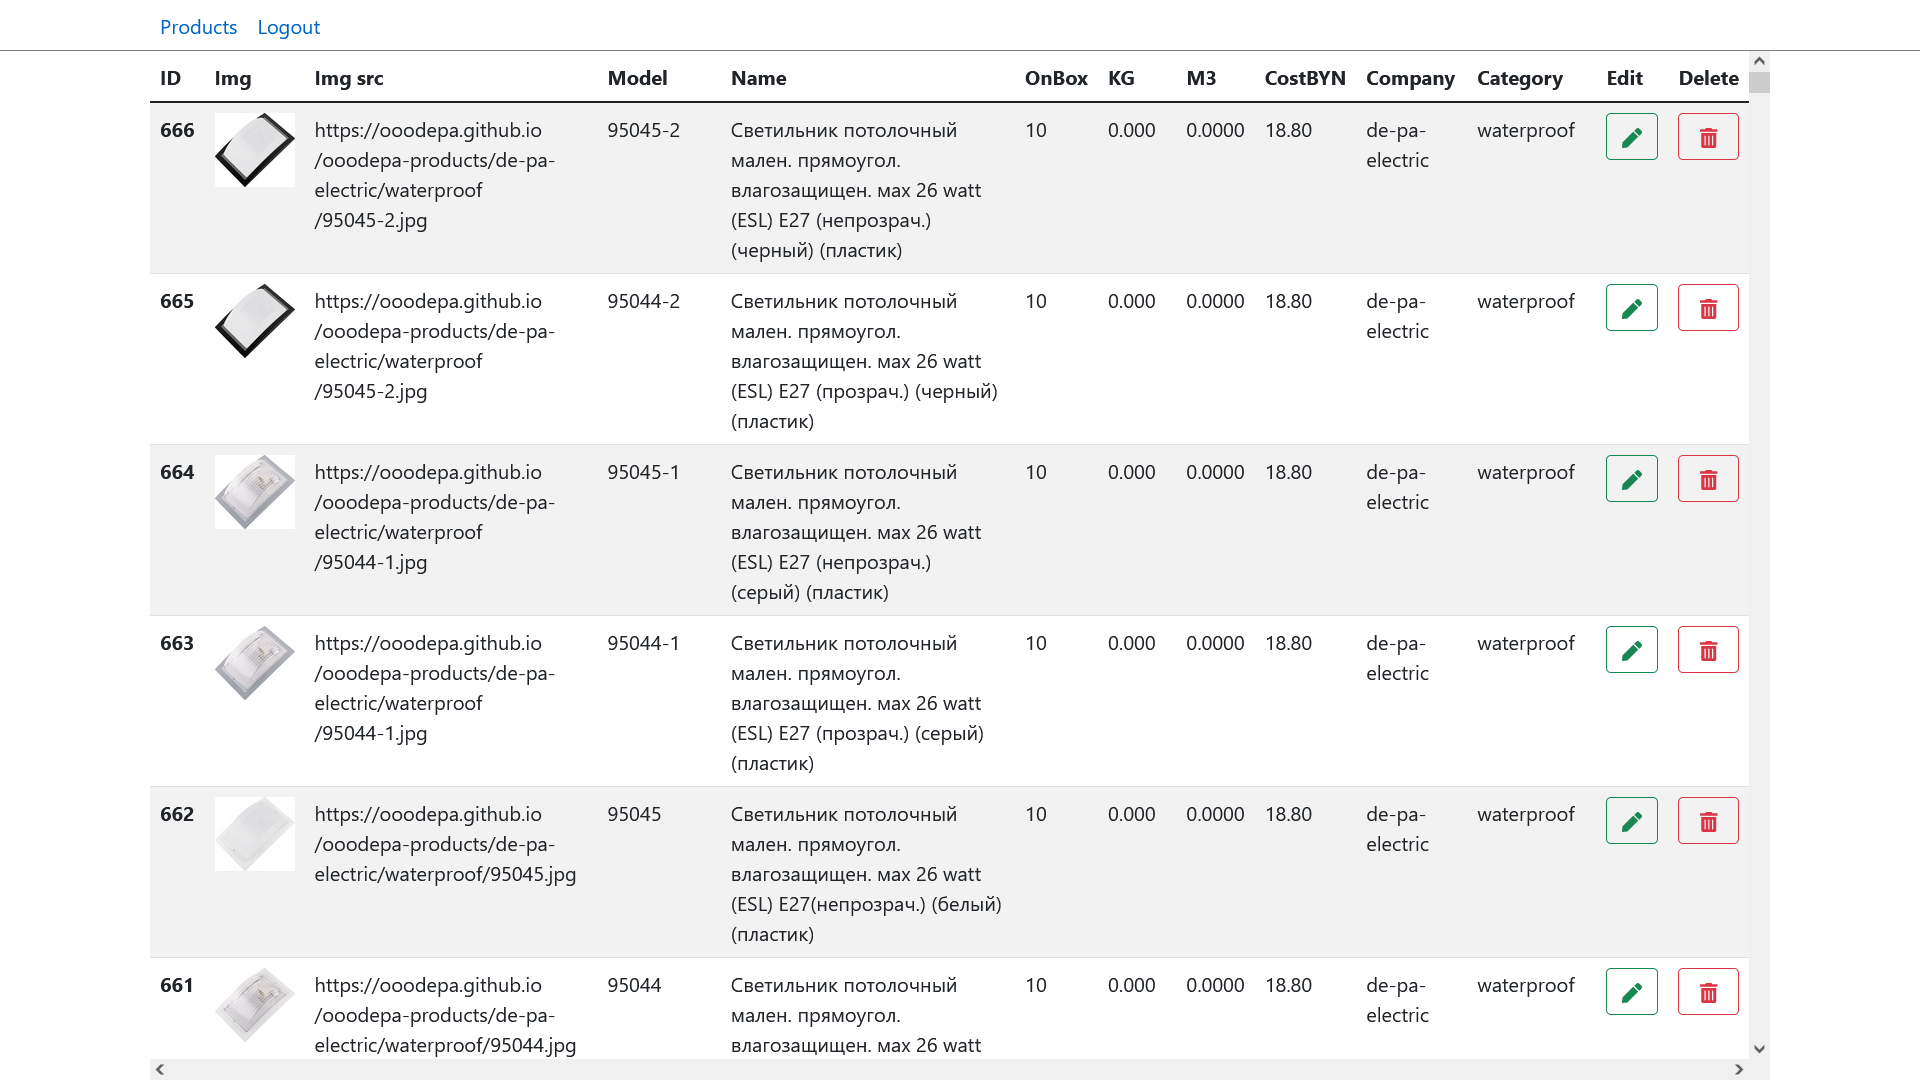
\includegraphics[width=12cm]
        {_assets/gpi_pz_not_empty_table.png}
    \caption{Таблица продуктов}
    \label{fig:gpi_pz_products_table}
\end{figure}

% = = = = = = = = = = = = = = = = = = = = = = = = = = = = = = = =

\subparagraph{Тестируемая задача:} <<Добавление нового продукта>>

\textit{Ожидаемый результат}: добавится новый продукт в БД. Данные можно увидеть в таблице продуктов.

\textit{Полученный результат}: получили сообщение о добавлении продукта. В таблице продуктов новые данные.

\textit{Выводы по тесту}: 
Скриншот соббщения о добавлении продукта на
\textbf{рис.~\ref{fig:gpi_pz_add_product} (стр.~\pageref{fig:gpi_pz_add_product})}.

\begin{figure}[!htb]
    \centering
    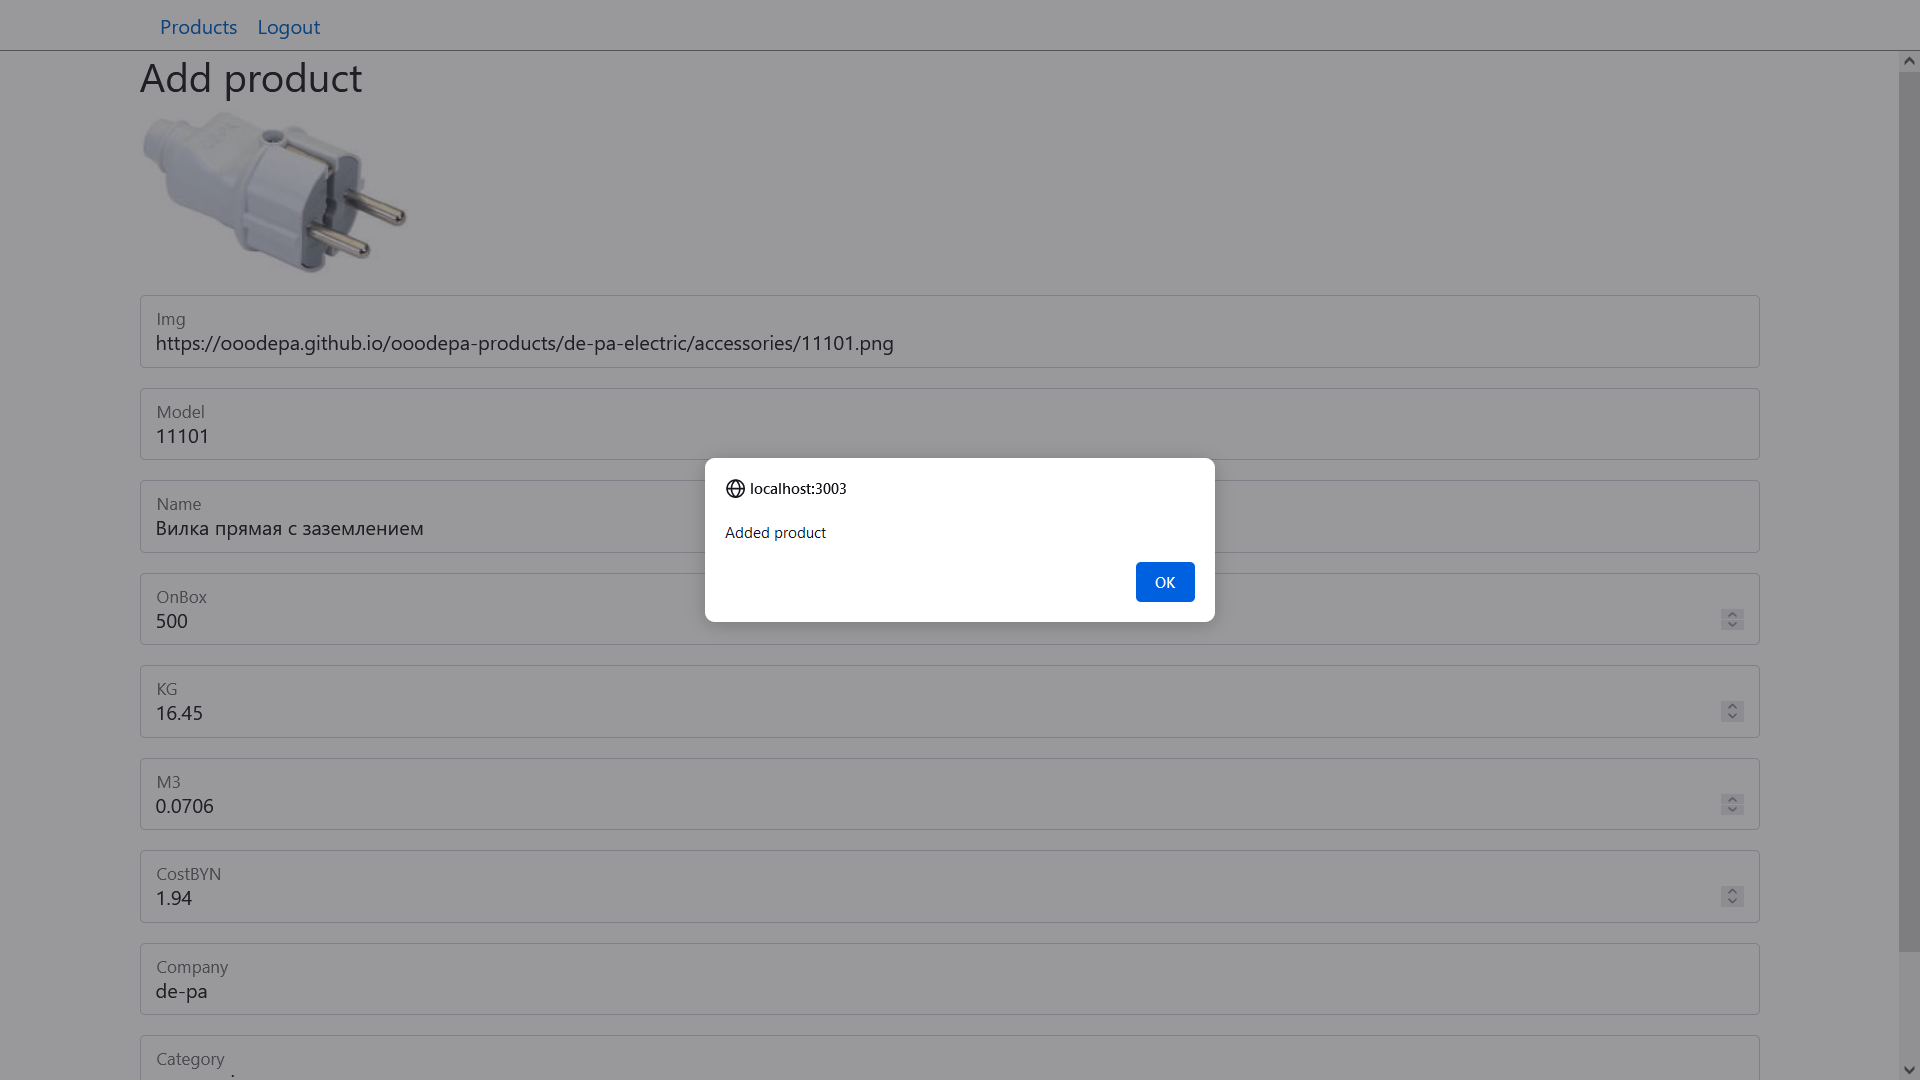
\includegraphics[width=12cm]
        {_assets/gpi_pz_add_product.png}
    \caption{Сообщение о добавлении продукта}
    \label{fig:gpi_pz_add_product}
\end{figure}

% = = = = = = = = = = = = = = = = = = = = = = = = = = = = = = = =

\subparagraph{Тестируемая задача:} <<Удаление продукта>>

\textit{Ожидаемый результат}: с таблицы удалится продукт.

\textit{Полученный результат}: продукт удалился с таблицы.

\textit{Выводы по тесту}: 
Скриншот сообщения об удалении продукта на
\textbf{рис.~\ref{fig:gpi_pz_delete_product} (стр.~\pageref{fig:gpi_pz_delete_product})}.

\begin{figure}[!htb]
    \centering
    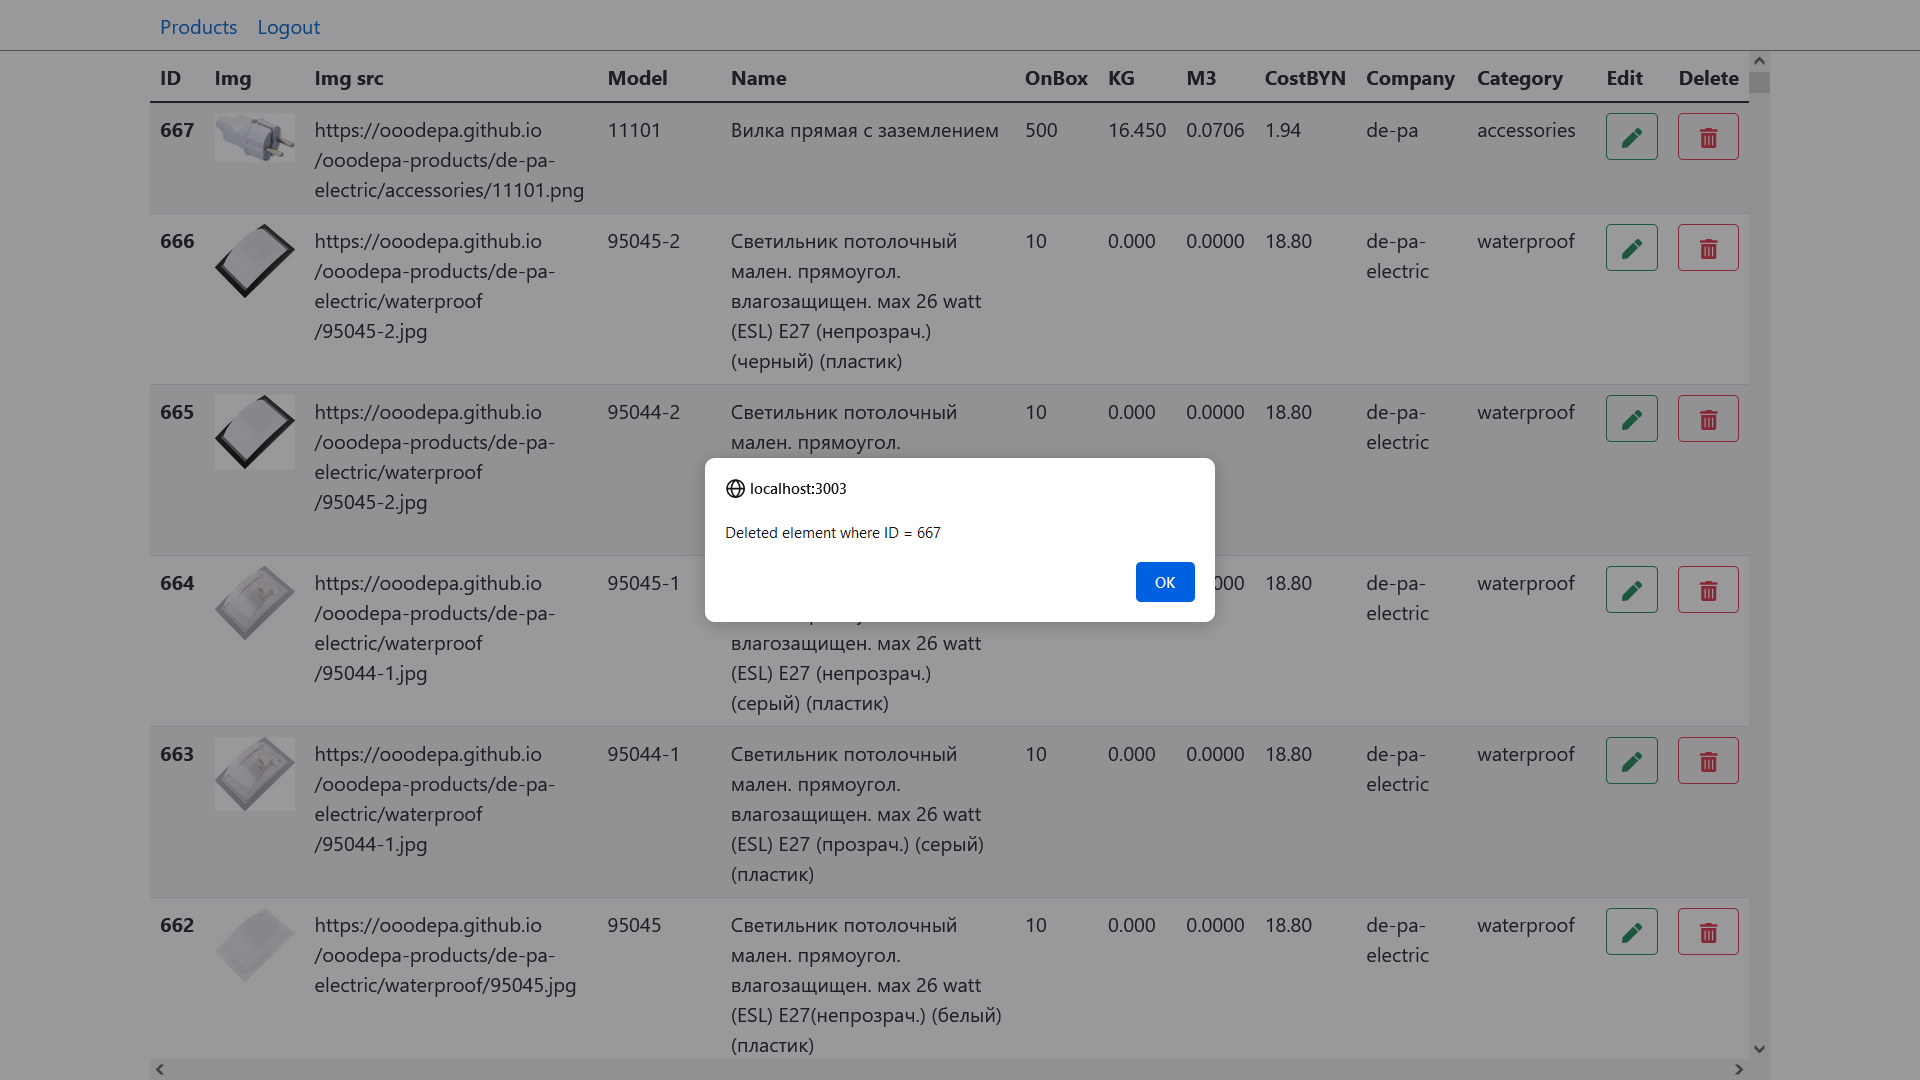
\includegraphics[width=12cm]
        {_assets/gpi_pz_delete_product.png}
    \caption{Сообщение о добавлении продукта}
    \label{fig:gpi_pz_delete_product}
\end{figure}

% = = = = = = = = = = = = = = = = = = = = = = = = = = = = = = = =

\subparagraph{Тестируемая задача:} <<Вывод продуктов для пользователя>>

\textit{Ожидаемый результат}: выведится сетка продуктов.

\textit{Полученный результат}: вывелась сетка продуктов.

\textit{Выводы по тесту}: 
Скриншот с продуктами для пользователя на
\textbf{рис.~\ref{fig:gpi_pz_user_products} (стр.~\pageref{fig:gpi_pz_user_products})}.

\begin{figure}[!htb]
    \centering
    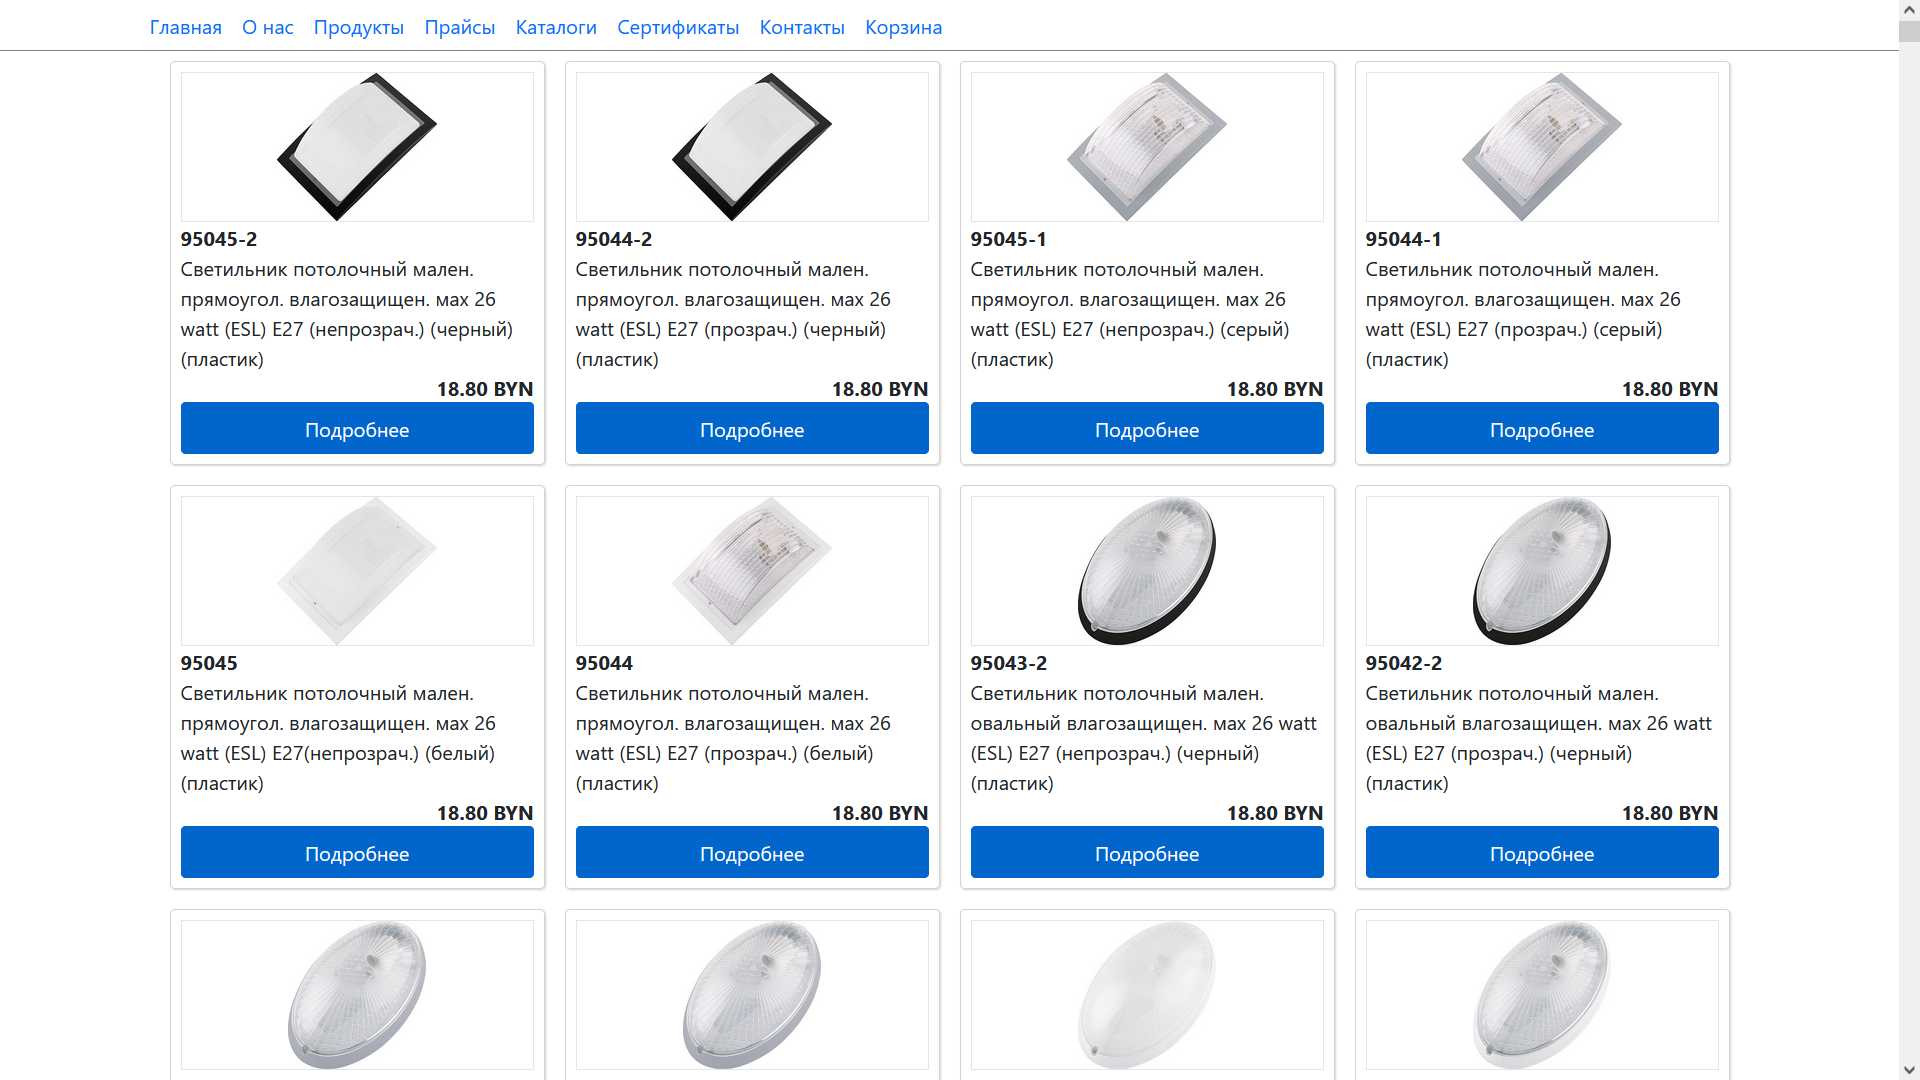
\includegraphics[width=16cm]
        {_assets/gpi_pz_user_products.png}
    \caption{Продукты для пользователя}
    \label{fig:gpi_pz_user_products}
\end{figure}

% = = = = = = = = = = = = = = = = = = = = = = = = = = = = = = = =

\subparagraph{Тестируемая задача:} <<Подробнее о товаре>>

\textit{Ожидаемый результат}: выведится подробная таблица с данными от продукте.

\textit{Полученный результат}: вывелась подробная таблица с данными о продукте.

\textit{Выводы по тесту}: 
Скриншот с таблицей данных о продукте на
\textbf{рис.~\ref{fig:gpi_pz_user_about_product} (стр.~\pageref{fig:gpi_pz_user_about_product})}.

\begin{figure}[!htb]
    \centering
    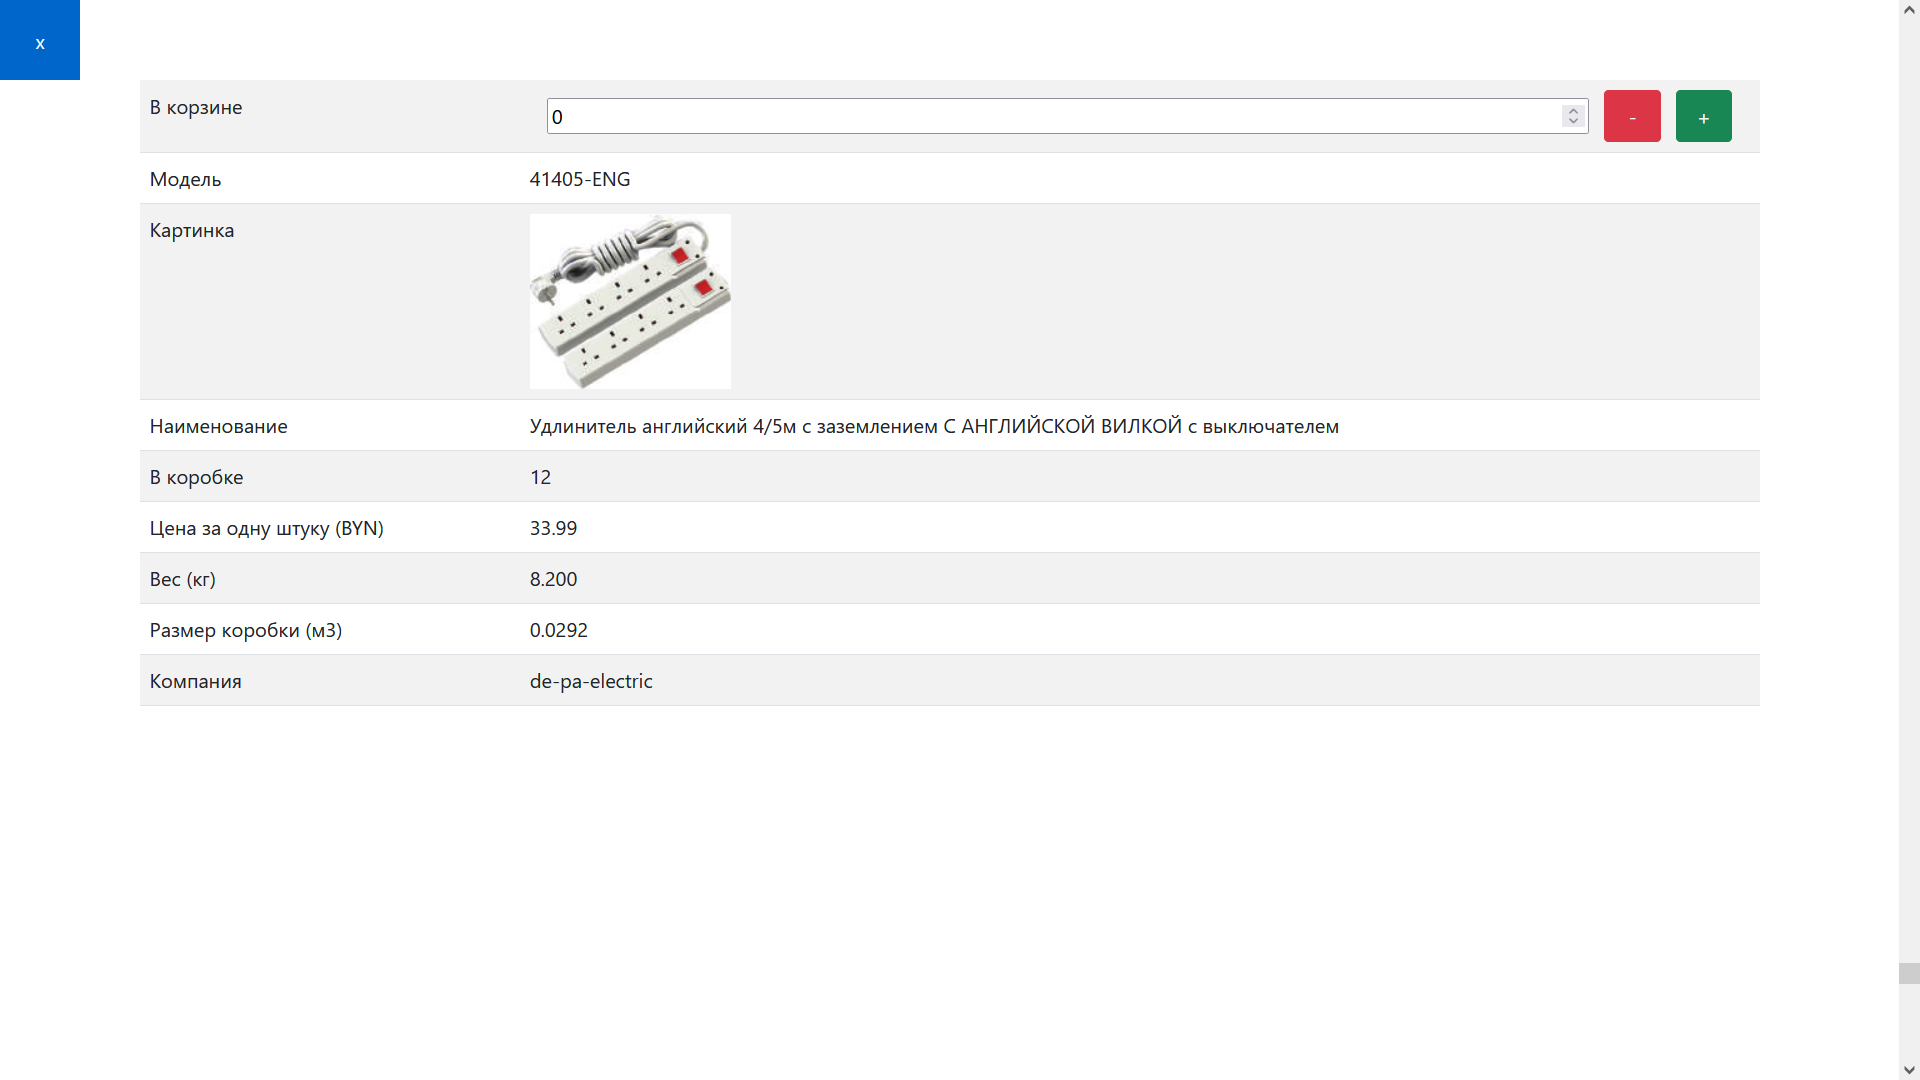
\includegraphics[width=14cm]
        {_assets/gpi_pz_user_about_product.png}
    \caption{Подробная таблица данных о продукте}
    \label{fig:gpi_pz_user_about_product}
\end{figure}

% = = = = = = = = = = = = = = = = = = = = = = = = = = = = = = = =

\subparagraph{Тестируемая задача:} <<Сохранение в корзину>>

\textit{Ожидаемый результат}: выбранные товары на сайте добавятся в корзину продуктов.

\textit{Полученный результат}: выбранные товары появились в корзине продуктов.

\textit{Выводы по тесту}: 
Скриншот с корзиной продуктов на
\textbf{рис.~\ref{fig:gpi_pz_backet} (стр.~\pageref{fig:gpi_pz_backet})}.

\begin{figure}[!htb]
    \centering
    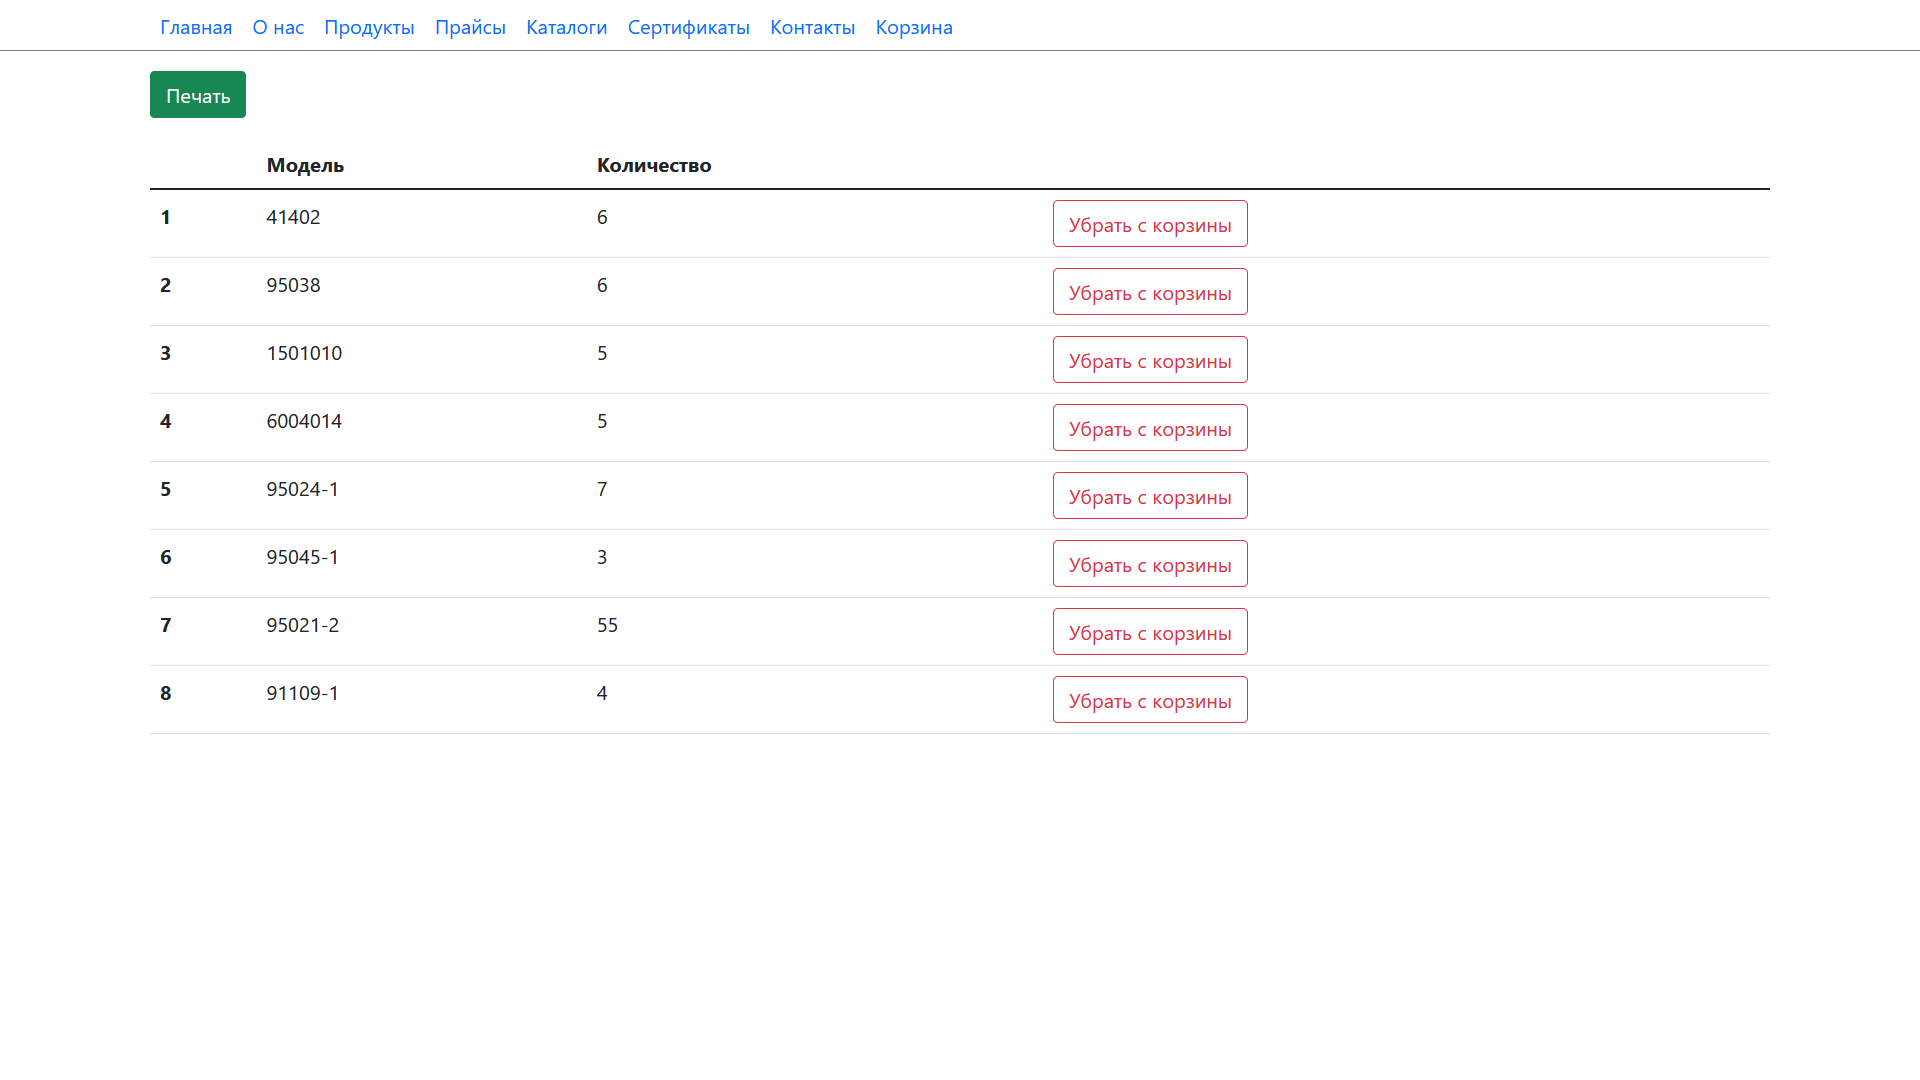
\includegraphics[width=14cm]
        {_assets/gpi_pz_backet.png}
    \caption{Корзина товаров}
    \label{fig:gpi_pz_backet}
\end{figure}

% = = = = = = = = = = = = = = = = = = = = = = = = = = = = = = = =

\newpage
